% Figure s04f01_ribbon (Session 4): the quantum Hall ribbon, its spectrum and its edges.
% The image is rendered by figures/blender/s04f01_ribbon.py; the coordinates of the labels come from
% figures/blender/out/s04f01_ribbon_anchors.tex. Build with figures/blender/build_figure.sh s04f01_ribbon.
\documentclass[11pt,tikz,border=0pt]{standalone}
\usepackage[T1]{fontenc}
\usepackage{amsmath,amssymb,graphicx,bm}
\usepackage{xcolor}
\usetikzlibrary{arrows.meta,calc}
% The three label colors of the figures, with the same values as in src/figures_preamble.tex.
\definecolor{aqmaccent}{RGB}{31,78,121}
\definecolor{aqmbroken}{RGB}{168,42,34}
\definecolor{aqmmuted}{RGB}{125,125,125}

% Shared TikZ styles of the overlays: axis arrows drawn on top of the renders, between anchors
% written by the scripts, so that they can be adjusted without rendering again.
\tikzset{
  axarrow/.style={line width=0.6pt, draw=black!70, -{Stealth[length=4.5pt,width=3.5pt]}},
  axlbl/.style={font=\small, inner sep=1.5pt},
}
% A discrete color key: \aqmkey{(x,y)}{color 1}{label 1}{color 2}{label 2} draws two swatches in a
% column with their labels, anchored at its north west corner. The colors are the sRGB values
% used in the render, defined below.
\definecolor{keypos}{RGB}{118,158,198}
\definecolor{keyneg}{RGB}{214,150,132}
\definecolor{keyup}{RGB}{224,62,40}
\definecolor{keydown}{RGB}{40,92,200}
\definecolor{keydark}{RGB}{31,78,121}
\definecolor{keylight}{RGB}{118,158,198}
\newcommand{\aqmkey}[5]{%
  \begin{scope}[shift={#1}]
    \fill[#2, draw=black!40, line width=0.3pt] (0,-0.32) rectangle (0.32,0);
    \node[font=\small, anchor=west, inner sep=1.5pt] at (0.38,-0.16) {#3};
    \fill[#4, draw=black!40, line width=0.3pt] (0,-0.74) rectangle (0.32,-0.42);
    \node[font=\small, anchor=west, inner sep=1.5pt] at (0.38,-0.58) {#5};
  \end{scope}}
% The same key in one row, for a figure with no room for a column.
\newcommand{\aqmkeyrow}[5]{%
  \begin{scope}[shift={#1}]
    \fill[#2, draw=black!40, line width=0.3pt] (0,-0.32) rectangle (0.32,0);
    \node[font=\small, anchor=west, inner sep=1.5pt] (k1) at (0.38,-0.16) {#3};
    \fill[#4, draw=black!40, line width=0.3pt] ([xshift=0.25cm]k1.east |- 0,-0.32) rectangle ++(0.32,0.32);
    \node[font=\small, anchor=west, inner sep=1.5pt] at ([xshift=0.63cm]k1.east) {#5};
  \end{scope}}

\newlength{\figw}\setlength{\figw}{15.6cm}   % the text width of the notes (A4, 2.7 cm margins)

\begin{document}
\begin{tikzpicture}[lbl/.style={font=\small, inner sep=1.5pt}, pnl/.style={font=\small\bfseries, inner sep=1.5pt}]
  \begin{scope}
    \setlength{\figw}{9.6cm}
    \node[overlay, anchor=south west, inner sep=0pt] at (0,0)
      {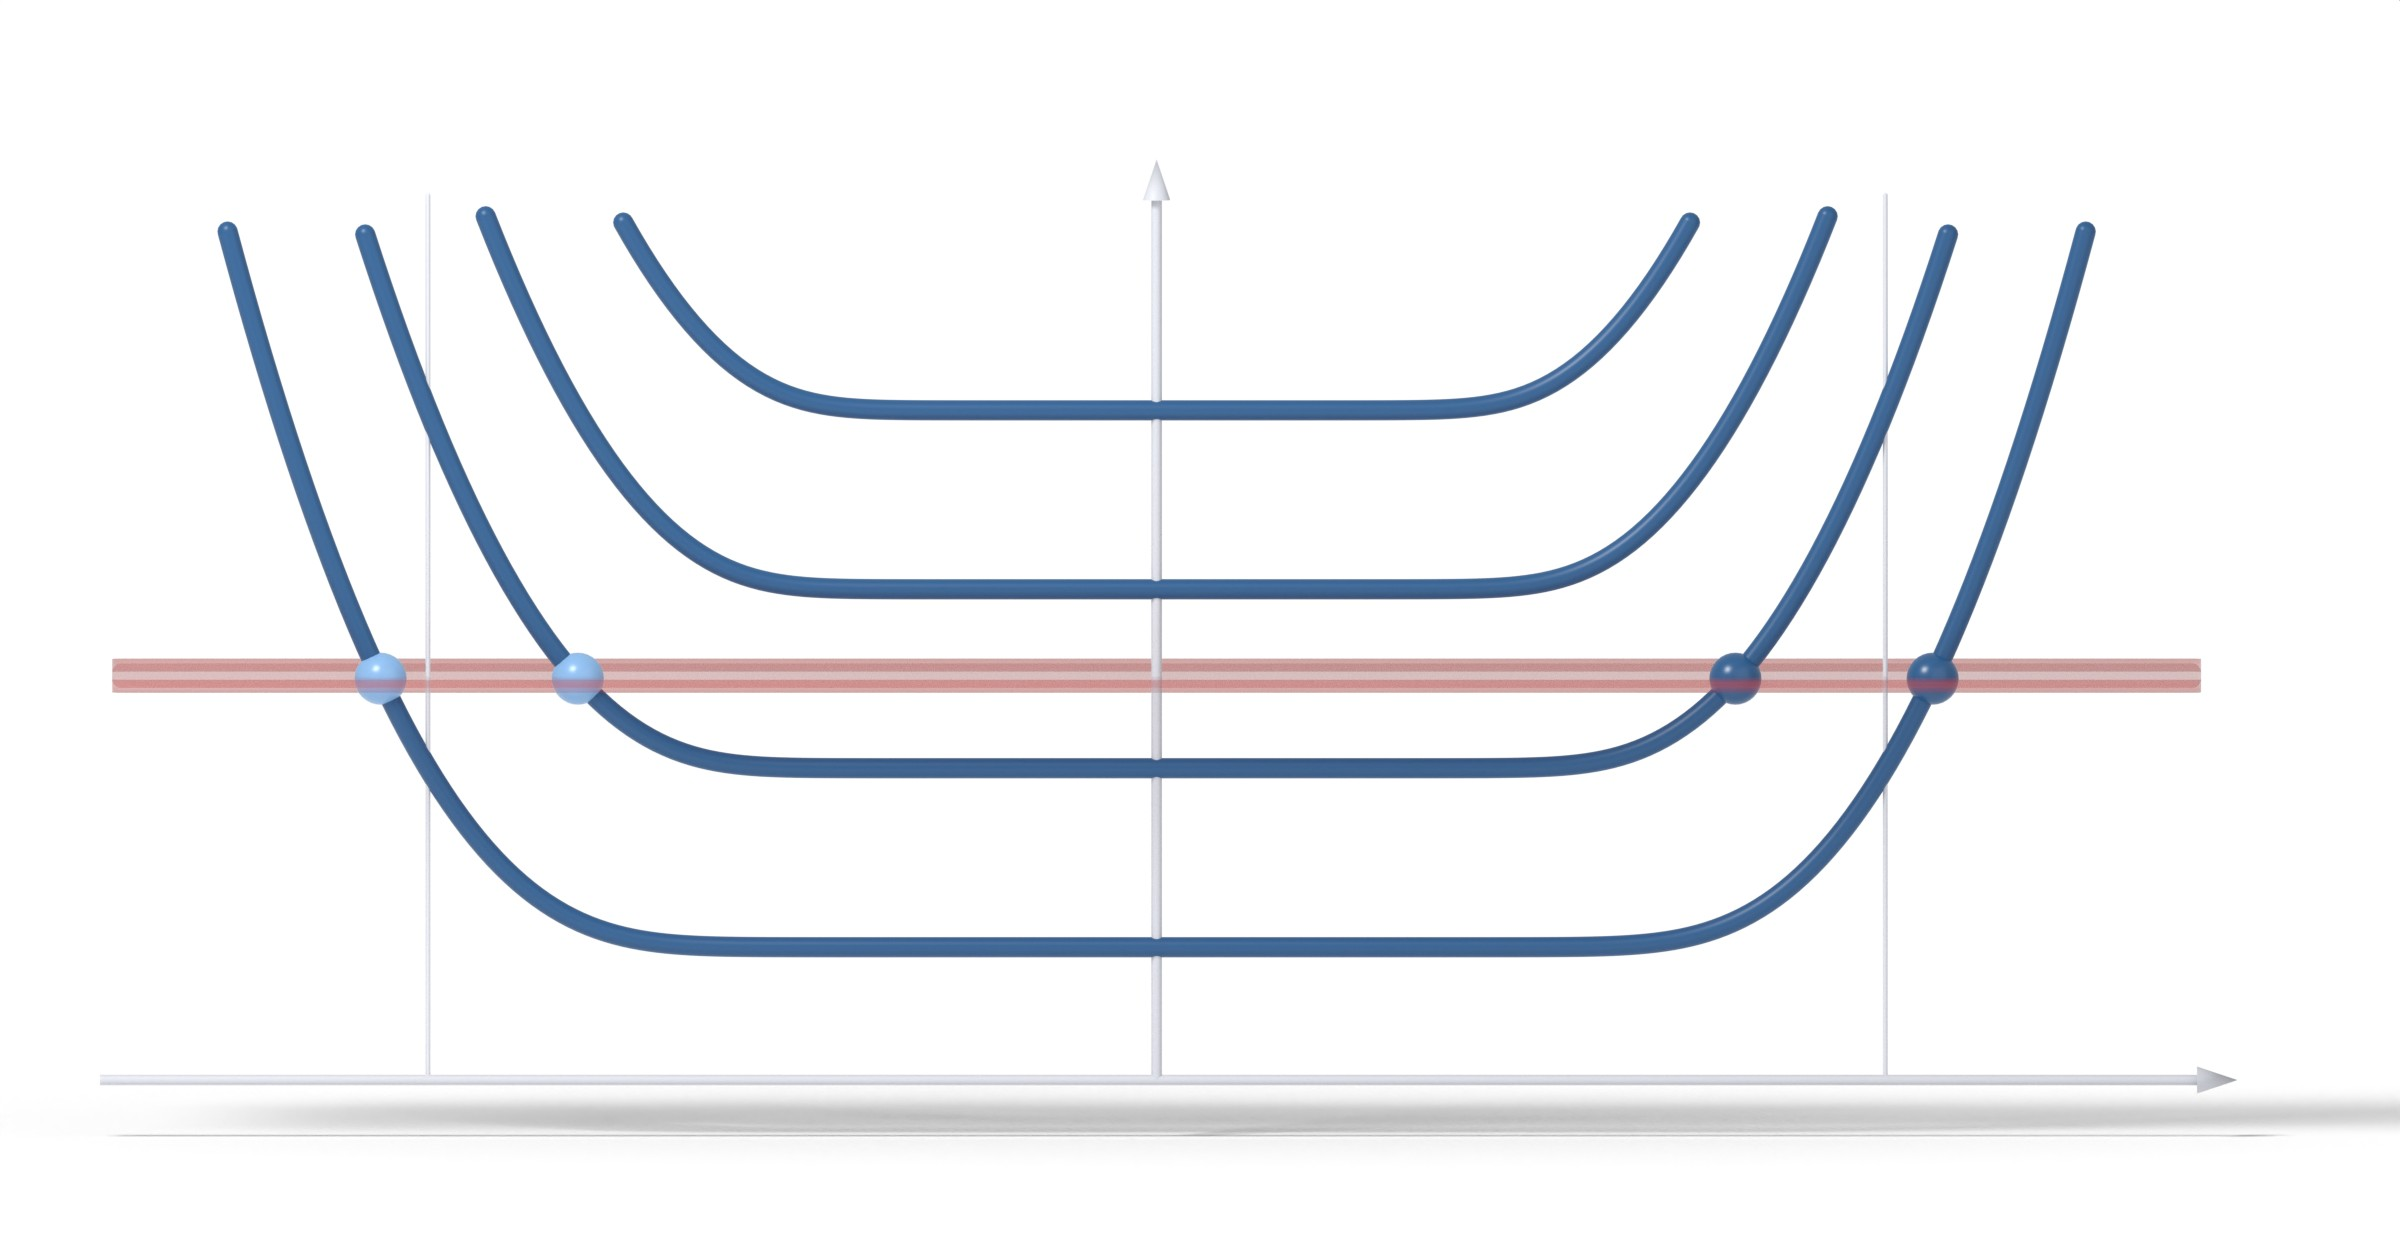
\includegraphics[width=\figw]{../blender/out/s04f01_ribbon_a.jpg}};
    % written by build_figure.sh; the painted part of the image
\path (0.0417\figw,0.0421\figw) rectangle (0.9988\figw,0.4542\figw);

    %% written by figlib.py; x and y in units of the image width
\coordinate (an0) at (0.4819\figw,0.1321\figw);
\coordinate (an1) at (0.4819\figw,0.2067\figw);
\coordinate (an2) at (0.4819\figw,0.2813\figw);
\coordinate (an3) at (0.4819\figw,0.3558\figw);
\coordinate (awallR) at (0.7855\figw,0.0665\figw);
\coordinate (awallL) at (0.1783\figw,0.0665\figw);
\coordinate (ak) at (0.9323\figw,0.0708\figw);
\coordinate (aE) at (0.4819\figw,0.4544\figw);
\coordinate (amu) at (0.9120\figw,0.2380\figw);
\coordinate (apanel) at (0.0316\figw,0.4432\figw);

    \node[pnl, anchor=south west] at (apanel) {(a)};
    \node[lbl, anchor=south east] at (ak) {$k_y$};
    \node[lbl, anchor=west] at (aE) {$E$};
    \node[lbl, anchor=north east, text=aqmbroken] at (amu) {$\mu$};
    \node[lbl, anchor=north, text=aqmmuted] at (awallL) {left wall};
    \node[lbl, anchor=north, text=aqmmuted] at (awallR) {right wall};
    \node[lbl, anchor=north, yshift=-2pt] at (an0) {$n=0$};
    \node[lbl, anchor=north, yshift=-2pt] at (an1) {$n=1$};
  \end{scope}
  \begin{scope}[shift={(9.8cm,0)}]
    \setlength{\figw}{5.8cm}
    \node[overlay, anchor=south west, inner sep=0pt] at (0,0)
      {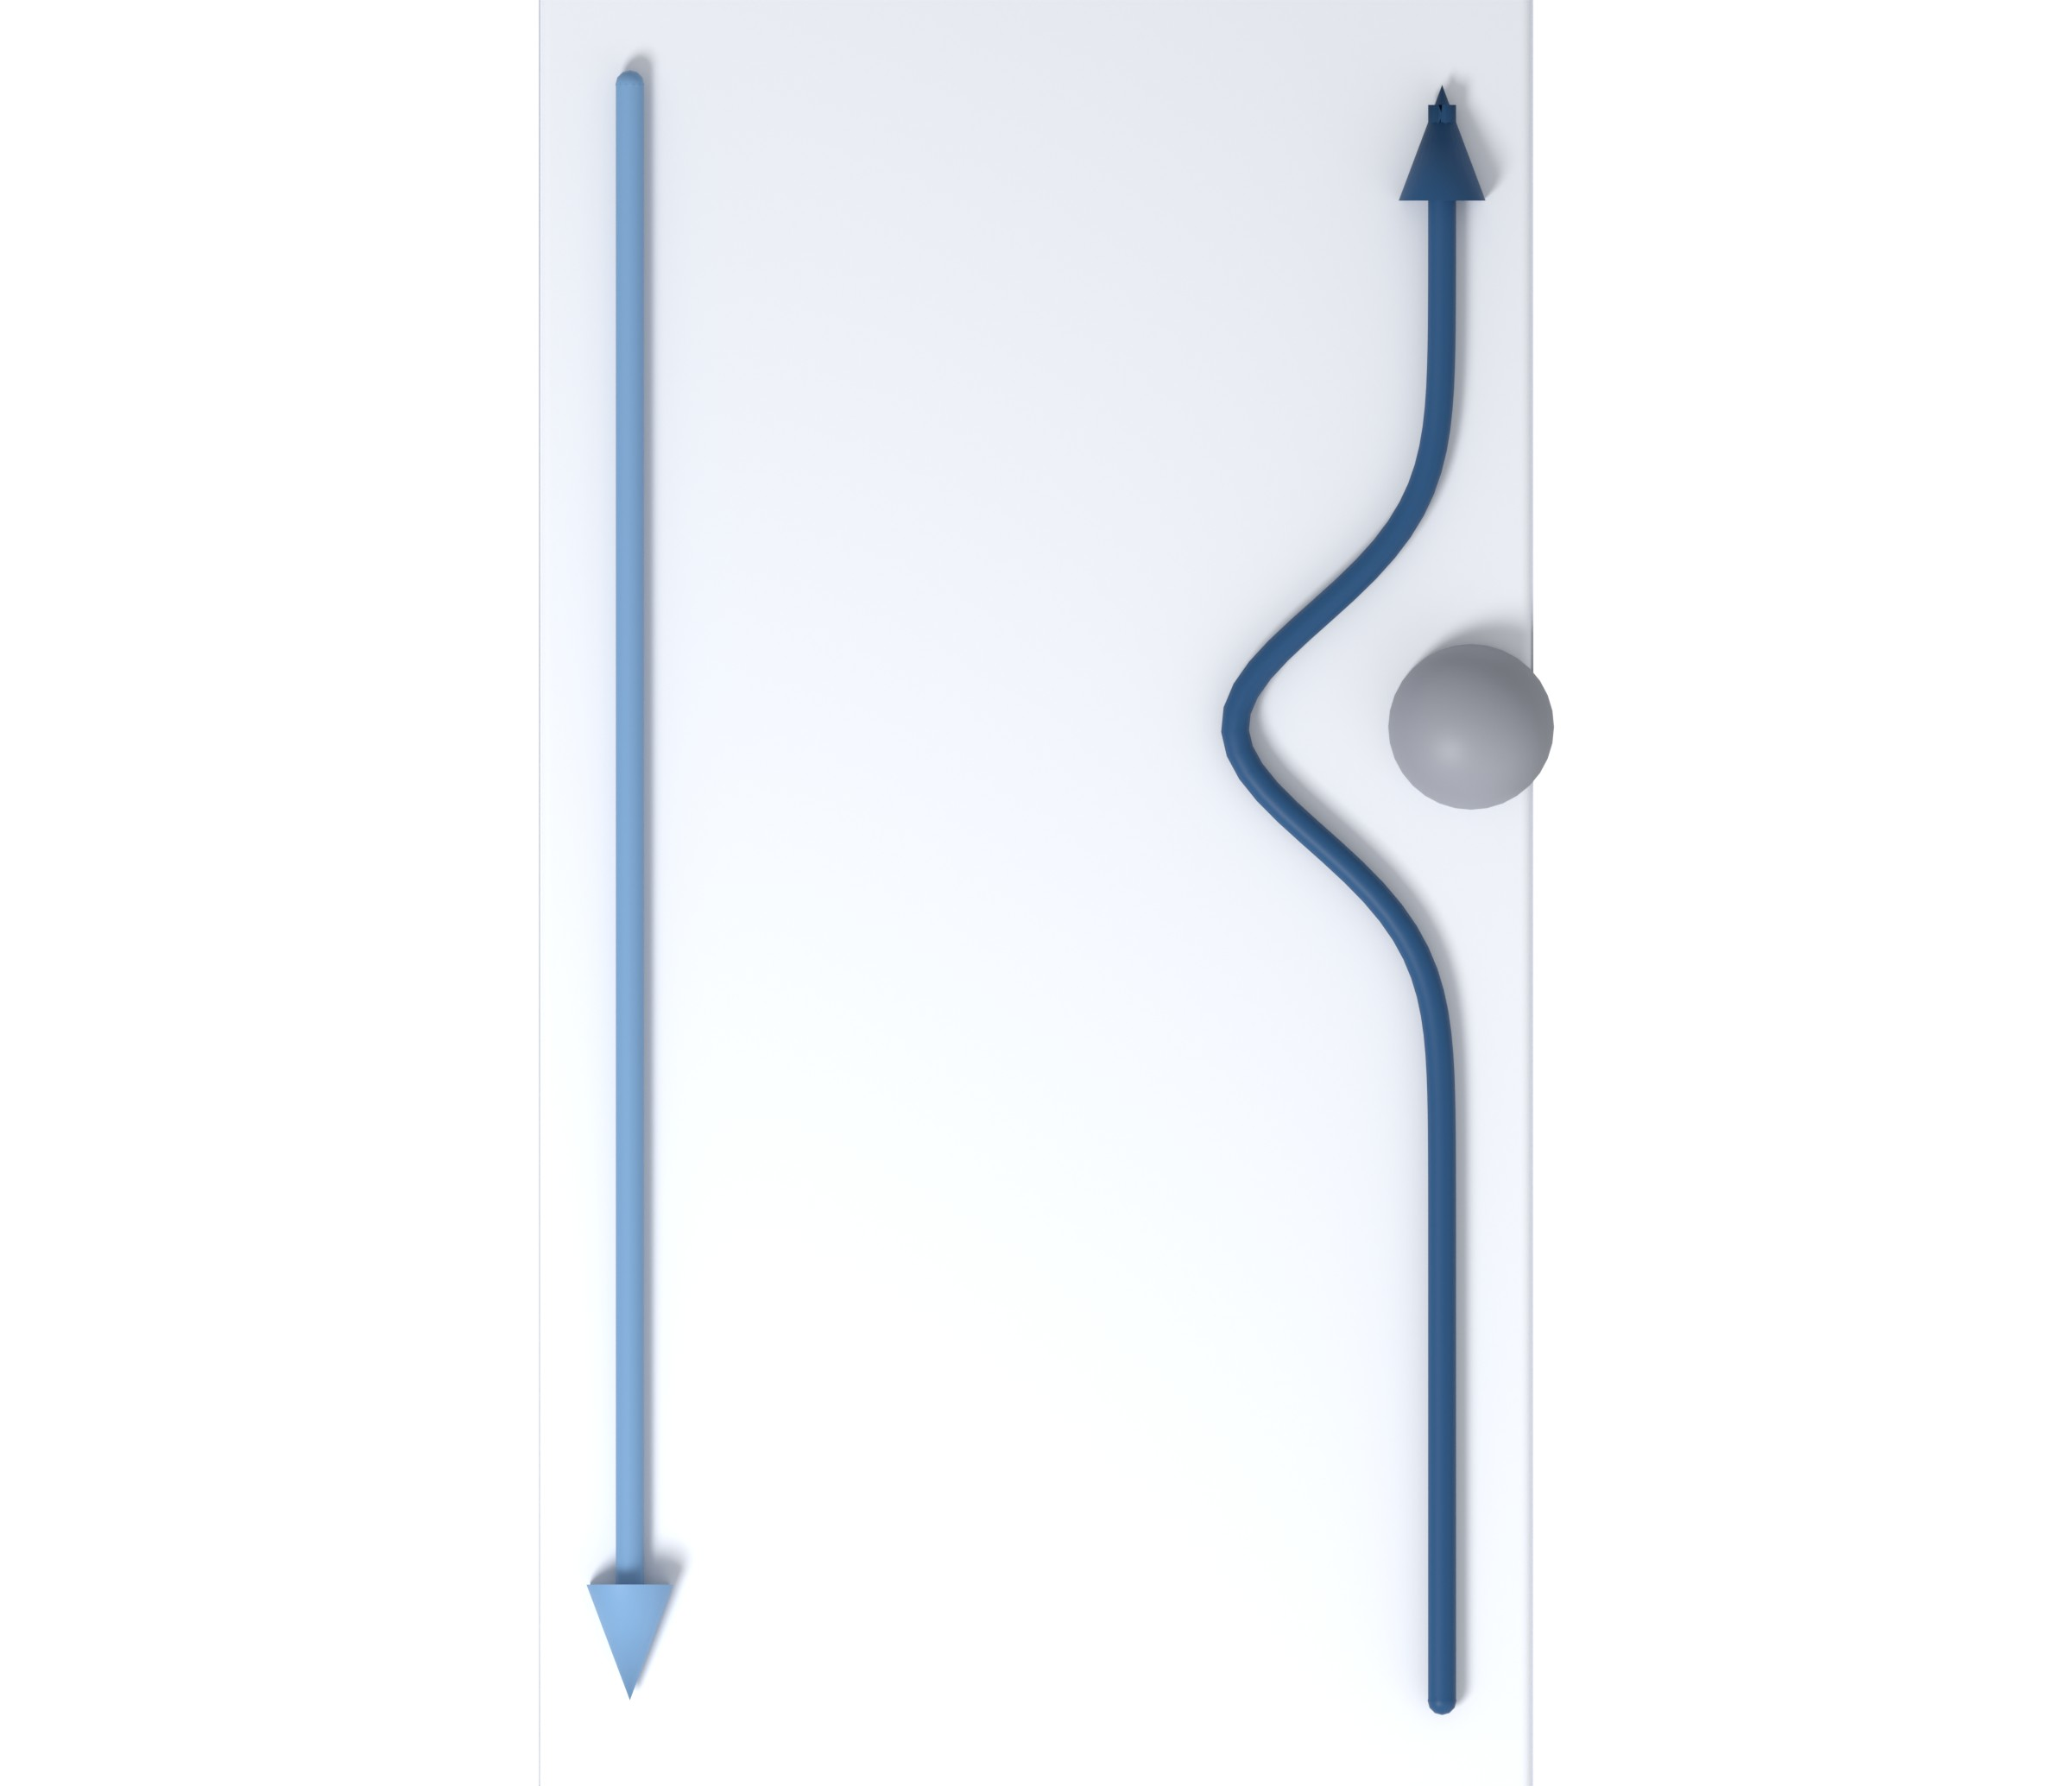
\includegraphics[width=\figw]{../blender/out/s04f01_ribbon_b.jpg}};
    % written by build_figure.sh; the painted part of the image
\path (0.2600\figw,0.0013\figw) rectangle (0.7504\figw,0.8608\figw);

    %% written by figlib.py; x and y in units of the image width
\coordinate (bimp) at (0.7500\figw,0.5112\figw);
\coordinate (bright) at (0.7400\figw,0.1112\figw);
\coordinate (bleft) at (0.2600\figw,0.1112\figw);
\coordinate (bpanel) at (0.0500\figw,0.8812\figw);
\coordinate (by) at (0.5000\figw,0.8712\figw);
\coordinate (brO) at (0.8100\figw,0.7012\figw);
\coordinate (brx) at (0.9500\figw,0.7012\figw);
\coordinate (bry) at (0.8100\figw,0.8412\figw);

    \node[pnl, anchor=north west] at (bpanel) {(b)};
    \node[lbl, anchor=west] at (bimp) {impurity};
    \node[lbl, anchor=west, align=left] at (bright) {$k_y>0$\\$v_y>0$};
    \node[lbl, anchor=east, align=right] at (bleft) {$k_y<0$\\$v_y<0$};
    \draw[axarrow] (brO) -- (brx);
  \draw[axarrow] (brO) -- (bry);
  \node[axlbl, anchor=north] at (brx) {$x$};
  \node[axlbl, anchor=east] at (bry) {$y$};
\end{scope}
\end{tikzpicture}
\end{document}
